\chapter{Les données}\label{chap:donnees}

La qualité d’un classifieur dépend d’abord de ses données. Ce chapitre décrit les jeux utilisés, la transformation en images recadrées par fruit, le découpage en trois ensembles et les choix destinés à limiter les biais~: pondération des classes et augmentation de données.

\section{Sources}

Nous avons combiné deux jeux de données publics, tous deux annotés au format YOLO~\cite{redmon2016} (une boîte englobante par fruit, avec sa classe de maturité)~:

\begin{itemize}
  \item un jeu de \textbf{bananes}~\cite{banane_ds} comportant 673 photographies, chacune annotée avec une seule boîte (sauf une image) et trois classes~: non mûre, mûre, trop mûre~;
  \item un jeu de \textbf{fraises et d’avocats}~\cite{dib2025}, comportant 758 photographies exploitables et huit classes (quatre stades pour chaque fruit~: non mûr, partiellement mûr, mûr, pourri). Les boîtes par classe vont de 48 à 260, et 708 images sur 758 ne contiennent qu’un seul fruit annoté.
\end{itemize}

Au total, nous disposons de \textbf{1\,431 photographies d’origine}. Les deux sources n’ont pas été prises dans les mêmes conditions (éclairage, fond, appareil), ce qui est à la fois une difficulté et un atout pour la robustesse.

\section{Les onze classes}

Le tableau~\ref{tab:classes} liste les classes finales. L’échelle de maturité n’est pas la même pour tous les fruits~: la banane a trois stades, la fraise et l’avocat en ont quatre, incluant un stade «~partiellement mûr~» intermédiaire et un stade «~pourri~».

\begin{table}[H]
\centering
\caption{Les 11 classes du projet et leur nombre d’images recadrées par ensemble.}\label{tab:classes}
\small
\begin{tabular}{@{}llrrrr@{}}
\toprule
\textbf{Fruit} & \textbf{Classe} & \textbf{Train} & \textbf{Val} & \textbf{Test} & \textbf{Total} \\
\midrule
\multirow{3}{*}{Banane} & non mûre & 154 & 33 & 33 & 220 \\
 & mûre & 144 & 30 & 31 & 205 \\
 & trop mûre & 174 & 38 & 37 & 249 \\
\midrule
\multirow{4}{*}{Fraise} & non mûre & 73 & 25 & 14 & 112 \\
 & partiellement mûre & 55 & 12 & 12 & 79 \\
 & mûre & 48 & 10 & 11 & 69 \\
 & pourrie & 68 & 14 & 6 & 88 \\
\midrule
\multirow{4}{*}{Avocat} & non mûr & 109 & 24 & 23 & 156 \\
 & partiellement mûr & 78 & 17 & 17 & 112 \\
 & mûr & 33 & 7 & 8 & 48 \\
 & pourri & 182 & 39 & 39 & 260 \\
\midrule
\multicolumn{2}{@{}l}{\textbf{Total}} & \textbf{1\,118} & \textbf{249} & \textbf{231} & \textbf{1\,598} \\
\bottomrule
\end{tabular}
\end{table}

Les effectifs sont nettement déséquilibrés~: la classe «~avocat pourri~» compte 260 images alors que «~avocat mûr~» n’en compte que 48. Pour les classes de fraises, le jeu de test ne contient parfois que 6 à 14 images, ce qui limite la précision des mesures par classe (chapitre~\ref{chap:resultats}).

\begin{figure}[H]
\centering
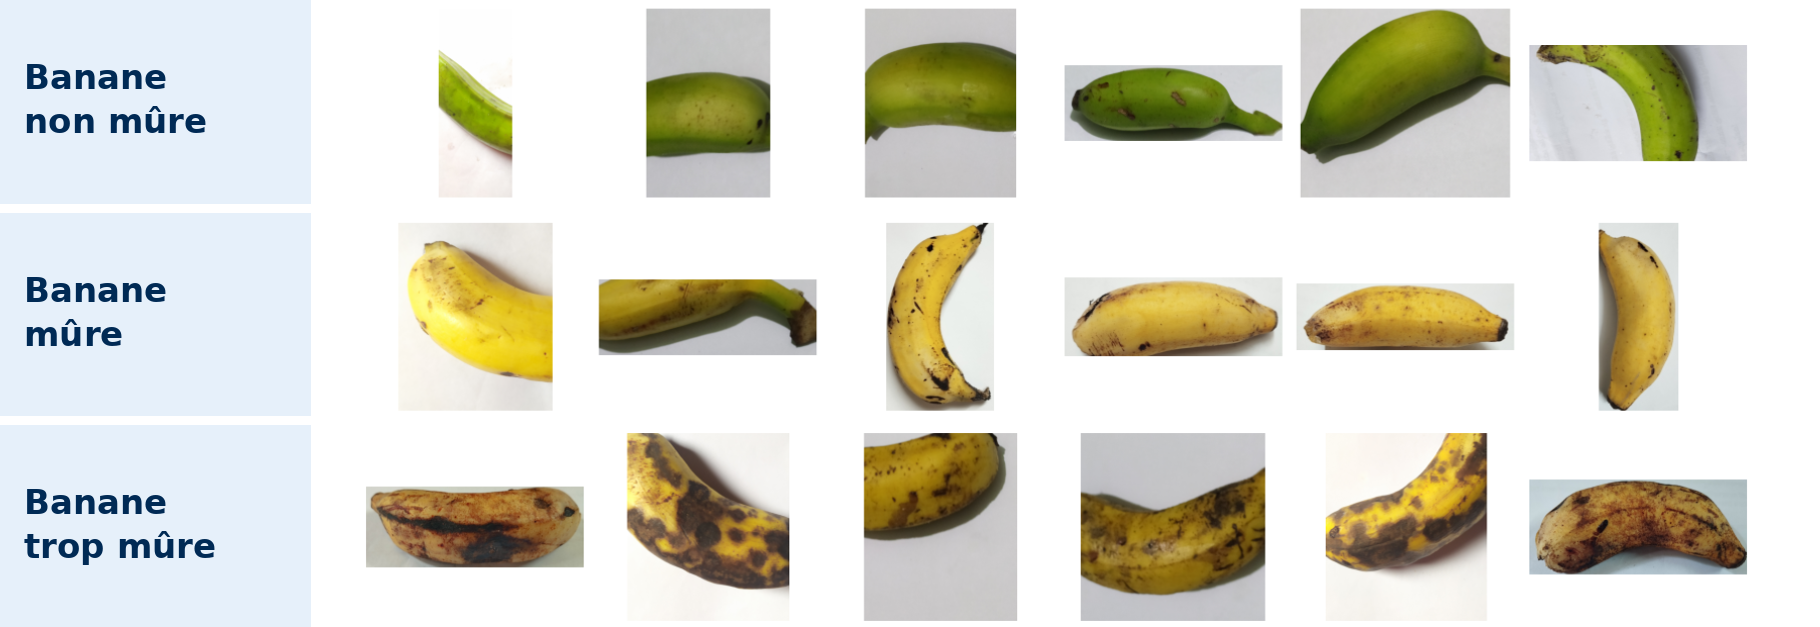
\includegraphics[width=0.9\textwidth]{figures/fig_ex_bananes.png}
\caption{Exemples de bananes recadrées, une ligne par stade de maturité.}
\end{figure}

\begin{figure}[H]
\centering
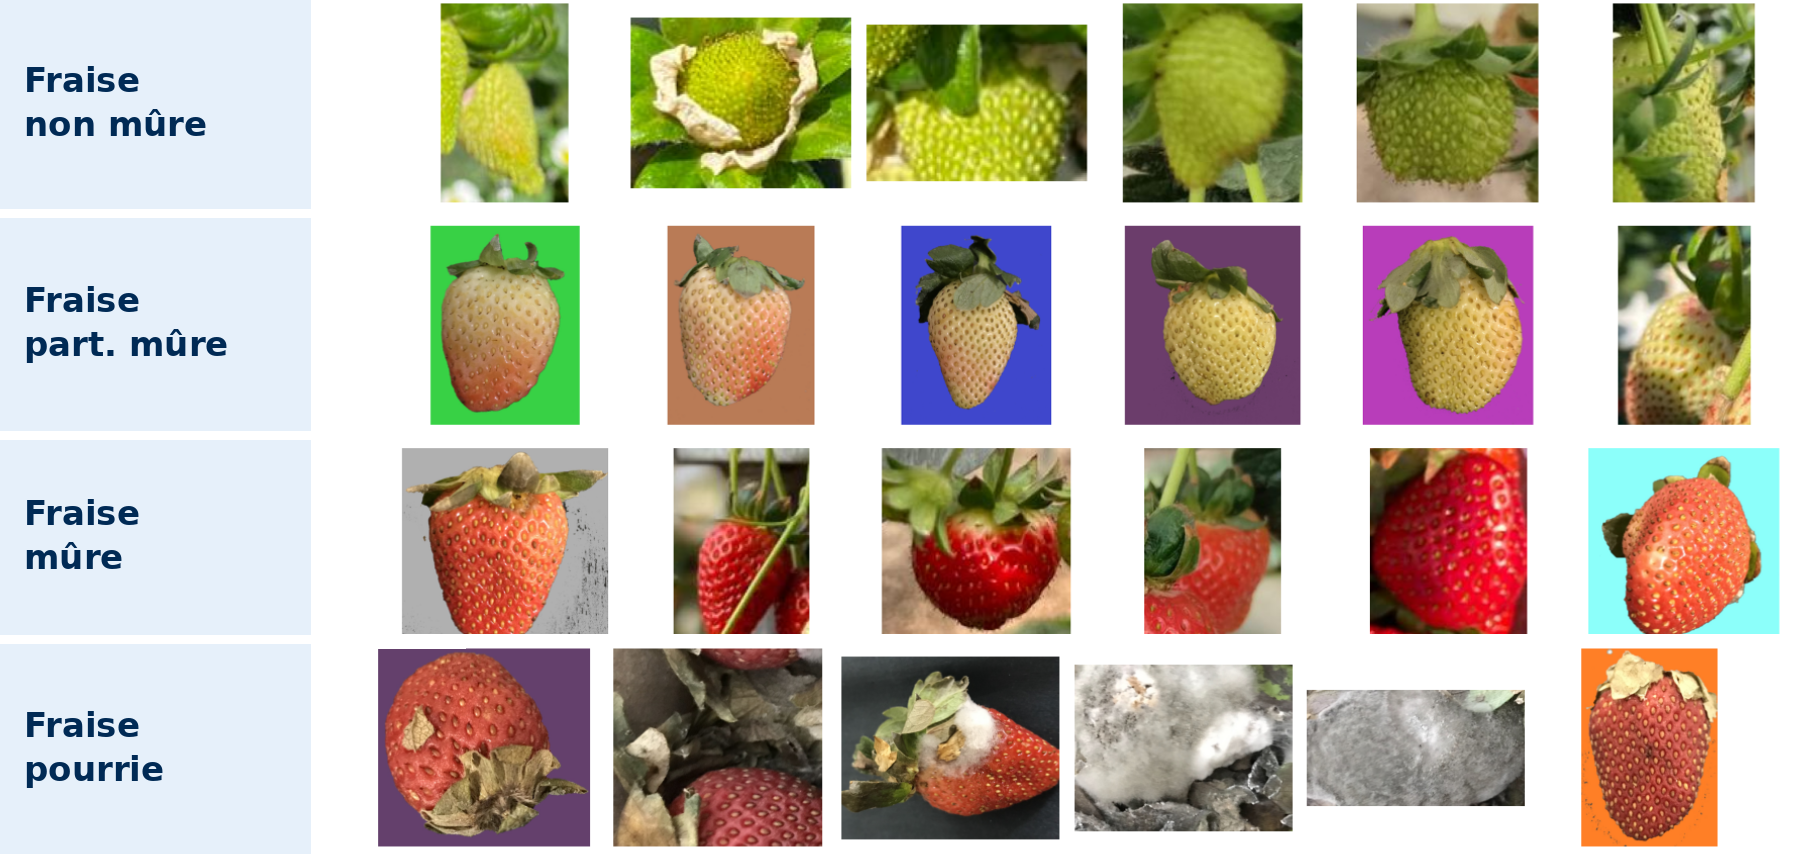
\includegraphics[width=0.9\textwidth]{figures/fig_ex_fraises.png}
\caption{Exemples de fraises recadrées, une ligne par stade, du stade non mûr au stade pourri.}
\end{figure}

\begin{figure}[H]
\centering
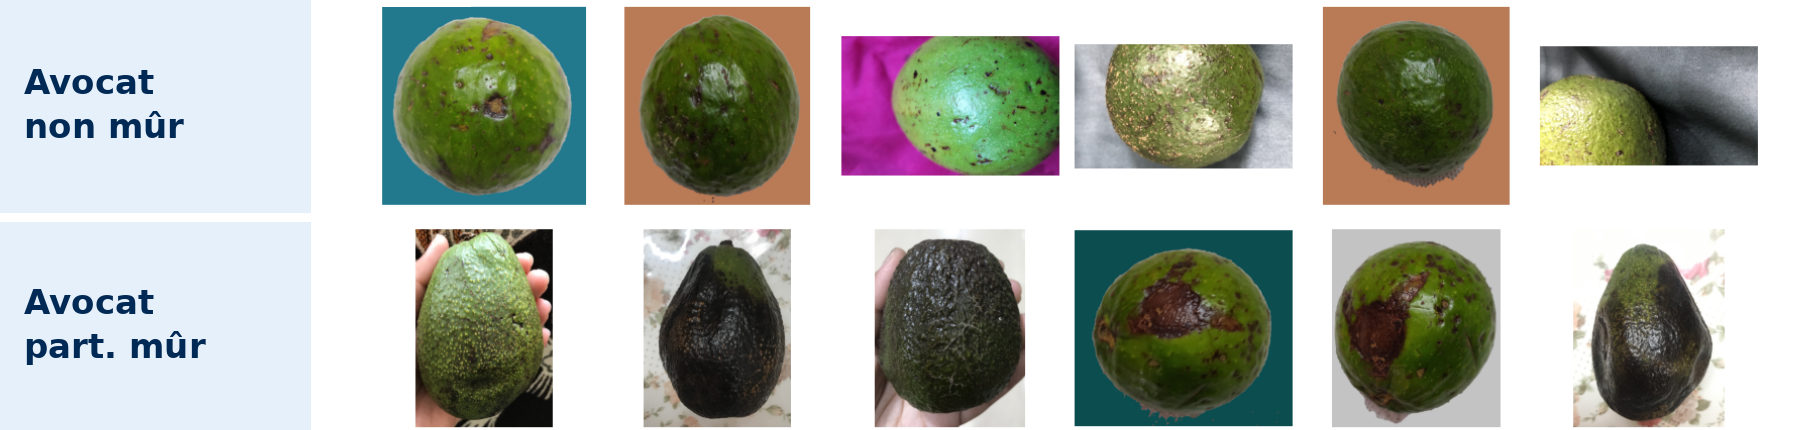
\includegraphics[width=0.9\textwidth]{figures/fig_ex_avocats.png}
\caption{Exemples d’avocats recadrés pour deux des quatre stades (non mûr et partiellement mûr).}
\end{figure}

\section{Recadrage à partir des boîtes}

Le classifieur reçoit une image d’un seul fruit. Nous recadrons donc chaque photographie selon les boîtes d’annotation. Chaque boîte YOLO est donnée par son centre $(x_c,y_c)$ et ses dimensions $(w,h)$, normalisés entre 0 et 1~; la boîte en pixels pour une image de taille $W\times H$ est~:
\begin{equation}
  x_{\min,\max} = \bigl(x_c \mp \tfrac{w’}{2}\bigr)\,W, \qquad y_{\min,\max} = \bigl(y_c \mp \tfrac{h’}{2}\bigr)\,H,
\end{equation}
avec $w’=1{,}05\,w$ et $h’=1{,}05\,h$ : nous ajoutons une \textbf{marge de 5\,\%} pour ne pas couper le bord du fruit, puis tronquons aux limites de l’image. Les boîtes de moins de \textbf{40 pixels} de côté sont ignorées, car elles ne contiennent pas assez d’information, et les recadrages sont réduits à 400 pixels maximum (miniature) pour limiter l’espace disque. Les 1\,431 photographies fournissent ainsi \textbf{1\,598 images de fruits}.

\section{Découpage sans fuite d’information}\label{sec:split}

Une même photographie peut contenir plusieurs fruits annotés. Si les recadrages d’une même photo étaient répartis entre entraînement et test, le modèle serait évalué sur des fruits voisins de ceux qu’il a vus~: c’est une \textbf{fuite d’information}, qui gonfle artificiellement la précision. Nous découpons donc \emph{par photographie d’origine} et non par recadrage~:

\begin{enumerate}
  \item chaque photo reçoit une étiquette égale à la classe majoritaire de ses boîtes~;
  \item les photos sont séparées en 70\,\% (entraînement), 15\,\% (validation) et 15\,\% (test) de façon \emph{stratifiée} sur cette étiquette, avec une graine fixée (\code{seed=42}) pour la reproductibilité ;
  \item chaque recadrage rejoint l’ensemble de sa photo.
\end{enumerate}

Le résultat est 1\,118 images d’entraînement, 249 de validation et 231 de test (tableau~\ref{tab:classes}). Le jeu de test n’est utilisé qu’à la fin pour mesurer les performances.

\begin{figure}[H]
\centering
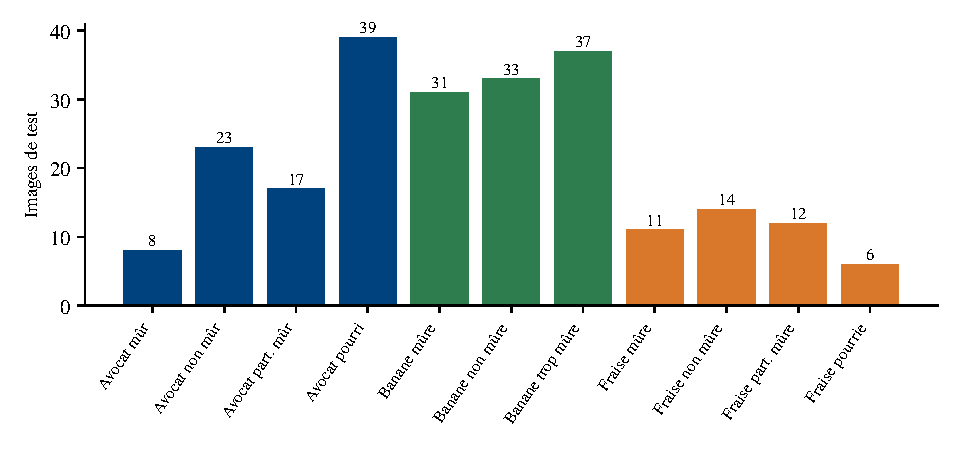
\includegraphics[width=0.78\textwidth]{figures/fig_support.pdf}
\caption{Nombre d’images de test par classe.}\label{fig:support}
\end{figure}

\section{Chaîne de chargement et prétraitement}

Les images sont lues par \code{image\_dataset\_from\_directory} de Keras, qui déduit les classes des noms de dossiers (ordre alphabétique), redimensionne à $224\times224$ pixels et forme des lots de 32 images. Les ensembles sont mis en préchargement (\code{prefetch}) pour recouvrir le calcul du GPU et le chargement des données.

Le prétraitement propre à MobileNetV2 (mise à l’échelle des pixels de $[0,255]$ vers $[-1,1]$, par une division suivie d’une soustraction) est intégré \emph{à l’intérieur du modèle}. Ce choix a un avantage décisif au déploiement~: l’application Android fournit directement les pixels bruts (valeurs 0--255) et n’a aucune normalisation à reproduire, ce qui supprime une source classique d’erreurs de décalage entre entraînement et production.

\section{Augmentation de données}

L’augmentation consiste à appliquer des transformations aléatoires aux images d’entraînement pour multiplier la diversité des exemples. Notre version retenue comprend~:

\begin{itemize}
  \item un retournement aléatoire horizontal et vertical (\code{RandomFlip})~;
  \item une rotation aléatoire jusqu’à $\pm 15\,\%$ d’un tour, soit $\pm 54^\circ$ (\code{RandomRotation})~;
  \item un zoom aléatoire de $\pm 15\,\%$ (\code{RandomZoom})~;
  \item une variation aléatoire de luminosité ($\pm 10\,\%$) et de contraste ($10\,\%$)~;
\end{itemize}

\begin{keybox}{Pas de changement de teinte}
Nous avons volontairement \emph{exclu} toute modification de la teinte (couleur)~: pour la maturité d’un fruit, la couleur est l’indice principal. Transformer du vert en jaune, ou du jaune en brun, changerait la classe de l’image sans changer son étiquette et brouillerait l’apprentissage.
\end{keybox}

Ces couches font partie du modèle mais ne sont actives qu’à l’entraînement~; la validation et le test utilisent les images telles quelles.

\section{Pondération des classes}\label{sec:poids}

Face au déséquilibre, un modèle naïf tend à favoriser les classes fréquentes. Nous attribuons à chaque classe un poids $\omega_k$ inversement proportionnel à sa fréquence, selon la formule «~balanced~» de scikit-learn~:
\begin{equation}
  \omega_k = \frac{N}{K\cdot n_k},
\end{equation}
où $N=1\,118$ est le nombre d’images d’entraînement, $K=11$ le nombre de classes et $n_k$ l’effectif de la classe $k$. Une erreur sur une classe rare coûte donc plus cher dans la perte. Les poids obtenus vont de \textbf{0,56} (avocat pourri, la plus fréquente) à \textbf{3,08} (avocat mûr, la plus rare)~; les trois classes de bananes, nombreuses, ont des poids compris entre 0,58 et 0,71.

\begin{table}[H]
\centering
\caption{Poids de classes utilisés dans la perte.}\label{tab:poids}
\small
\begin{tabular}{@{}lrlr@{}}
\toprule
\textbf{Classe} & $\omega_k$ & \textbf{Classe} & $\omega_k$ \\
\midrule
avocat mûr & 3,08 & banane mûre & 0,71 \\
fraise mûre & 2,12 & banane non mûre & 0,66 \\
fraise partiellement mûre & 1,85 & banane trop mûre & 0,58 \\
fraise pourrie & 1,49 & avocat non mûr & 0,93 \\
fraise non mûre & 1,39 & avocat pourri & 0,56 \\
avocat partiellement mûr & 1,30 & & \\
\bottomrule
\end{tabular}
\end{table}

Cette pondération améliore le rappel des classes rares au prix d’une légère baisse de précision sur les classes fréquentes, compromis jugé acceptable~: une fraise mûre manquée est plus gênante qu’une hésitation sur une banane.
